\section{Birefringence}
Birefringence is a physical phenomena which was observed for the first time in calcite crystals, by the Danish scientist Rasmus Bartholin in 1669 \cite{RasmusBartholin1669ExperimentaDetegitur}. The effect of birefringence is relatively easy to show. One can simply place a birefringent crystal on top of some text, as it is shown in figure \ref{fig:3birefringence}. Two images of the text become visible through the crystal and each image is shifted by a different amount. These images are not simply reflections at the crystal-air interface. Since the images are brighter compared to images formed through reflections, and they are even visible when looking down directly from above. Also if the crystal is rotated then one of the pictures will be stationary, while the other one will move around the stationary image. The same effect can be illustrated by sending an unpolarized laser beam through the crystal. The beam is split in two as it propagates through the crystal. \cite{Roth2019Optik}

\begin{figure}
    \centering
    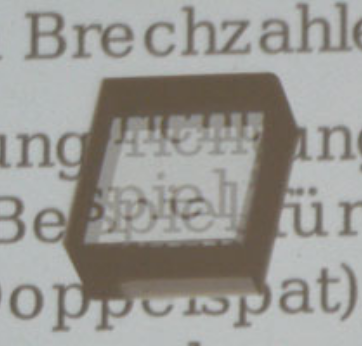
\includegraphics[scale=0.35]{images/3_chapter03/birefringence.png}
    \caption{A calcite crystal placed on top of some text. This demonstrates the effect of birefringence on the original image seen through the crystal. \cite{Roth2019Optik}}
    \label{fig:3birefringence}
\end{figure}

\subsection{Natural}

\subsection{Form birefringence}

\section{Waveplates}

\section{Jones calculus}

\section{Mueller calculus}

\section{Uniaxial media boundary conditions}

\section{Optimization?}
- describe algorithm
